\documentclass[11pt,a4paper]{article}

% -------------------------------------------------------
% Packages
% -------------------------------------------------------
\usepackage[T1]{fontenc}
\usepackage[utf8]{inputenc}
\usepackage{lmodern}
\usepackage{geometry}
\geometry{margin=2.5cm}

\usepackage{hyperref}
\hypersetup{
    colorlinks=true,
    linkcolor=blue!70!black,
    urlcolor=blue!70!black,
    citecolor=green!50!black,
}

\usepackage{xcolor}
\definecolor{codebg}{HTML}{F5F5F5}
\definecolor{framecolor}{HTML}{CCCCCC}
\definecolor{keywordcolor}{HTML}{0000CC}
\definecolor{commentcolor}{HTML}{008000}
\definecolor{stringcolor}{HTML}{CC0000}
\definecolor{tikzblue}{HTML}{2196F3}
\definecolor{tikzgreen}{HTML}{4CAF50}
\definecolor{tikzorange}{HTML}{FF9800}
\definecolor{tikzred}{HTML}{F44336}
\definecolor{tikzpurple}{HTML}{9C27B0}

\usepackage{listings}
\lstdefinestyle{python}{
    language=Python,
    backgroundcolor=\color{codebg},
    frame=single,
    rulecolor=\color{framecolor},
    basicstyle=\ttfamily\footnotesize,
    keywordstyle=\color{keywordcolor}\bfseries,
    commentstyle=\color{commentcolor}\itshape,
    stringstyle=\color{stringcolor},
    showstringspaces=false,
    breaklines=true,
    numbers=left,
    numberstyle=\tiny\color{gray},
    numbersep=8pt,
    tabsize=4,
    captionpos=b,
}
\lstdefinestyle{bash}{
    language=bash,
    backgroundcolor=\color{codebg},
    frame=single,
    rulecolor=\color{framecolor},
    basicstyle=\ttfamily\footnotesize,
    keywordstyle=\color{keywordcolor}\bfseries,
    commentstyle=\color{commentcolor}\itshape,
    showstringspaces=false,
    breaklines=true,
    captionpos=b,
}
\lstdefinestyle{yaml}{
    backgroundcolor=\color{codebg},
    frame=single,
    rulecolor=\color{framecolor},
    basicstyle=\ttfamily\footnotesize,
    breaklines=true,
    captionpos=b,
}

\usepackage{booktabs}
\usepackage{array}
\usepackage{tabularx}
\usepackage{tikz}
\usetikzlibrary{shapes.geometric, arrows.meta, positioning, trees, fit, backgrounds}

\usepackage{graphicx}
\usepackage{caption}
\usepackage{subcaption}
\usepackage{enumitem}
\usepackage{parskip}
\usepackage{microtype}
\usepackage{amsmath}

% -------------------------------------------------------
% Title
% -------------------------------------------------------
\title{%
    \textbf{Custom Training Guide}\\[6pt]
    \large MediaPipe EfficientDet-Lite2 with 150 Custom Classes
}
\author{MediaPipe Custom Training Pipeline}
\date{\today}

% -------------------------------------------------------
\begin{document}
% -------------------------------------------------------

\maketitle
\tableofcontents
\newpage

% -------------------------------------------------------
\section{Introduction}
% -------------------------------------------------------

This document provides a comprehensive guide to training a MediaPipe
\textbf{EfficientDet-Lite2} object-detection model on \textbf{150 custom classes
from scratch}. It covers every stage of the pipeline: data collection,
annotation, TFRecord conversion, model training, evaluation, and TFLite export
for on-device inference.

% -------------------------------------------------------
% TikZ Flowchart: Pipeline Overview
% -------------------------------------------------------
\subsection{Pipeline Overview}

\begin{figure}[ht]
\centering
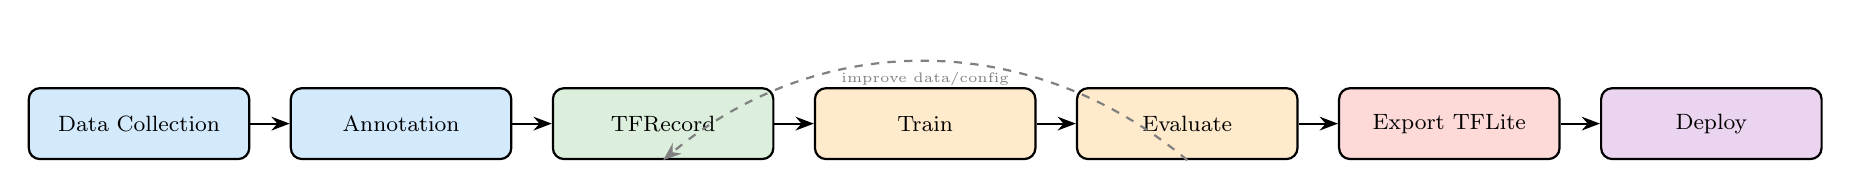
\begin{tikzpicture}[
    node distance=1.6cm and 0.5cm,
    box/.style={
        rectangle, rounded corners=4pt, draw, thick,
        minimum width=2.8cm, minimum height=0.9cm,
        text centered, font=\footnotesize
    },
    arr/.style={-Stealth, thick}
]

\node[box, fill=tikzblue!20]   (collect)   {Data Collection};
\node[box, fill=tikzblue!20,   right=of collect]  (annotate)  {Annotation};
\node[box, fill=tikzgreen!20,  right=of annotate] (tfrecord)  {TFRecord};
\node[box, fill=tikzorange!20, right=of tfrecord] (train)     {Train};
\node[box, fill=tikzorange!20, right=of train]    (evaluate)  {Evaluate};
\node[box, fill=tikzred!20,    right=of evaluate] (export)    {Export TFLite};
\node[box, fill=tikzpurple!20, right=of export]   (deploy)    {Deploy};

\draw[arr] (collect)  -- (annotate);
\draw[arr] (annotate) -- (tfrecord);
\draw[arr] (tfrecord) -- (train);
\draw[arr] (train)    -- (evaluate);
\draw[arr] (evaluate) -- (export);
\draw[arr] (export)   -- (deploy);

% Feedback loop
\draw[arr, dashed, bend right=40, color=gray]
    (evaluate.south) to node[below, font=\tiny]{improve data/config} (tfrecord.south);

\end{tikzpicture}
\caption{End-to-end training pipeline. The dashed arrow shows the iterative
         improvement loop: evaluation findings feed back into data collection
         and configuration refinement.}
\label{fig:pipeline}
\end{figure}

% -------------------------------------------------------
\section{Prerequisites}
% -------------------------------------------------------

\begin{itemize}[nosep]
    \item Python 3.9 or 3.10
    \item CUDA 11.8 + cuDNN 8.6
    \item NVIDIA GPU with at least 16\,GB VRAM
    \item 32\,GB system RAM (64\,GB preferred)
    \item 500\,GB SSD free space
\end{itemize}

% -------------------------------------------------------
\section{Step 1: Setting Up the Environment}
% -------------------------------------------------------

\begin{lstlisting}[style=bash, caption={Create virtual environment and install dependencies}]
python3.10 -m venv .venv
source .venv/bin/activate
pip install --upgrade pip
pip install -r requirements/python_requirements.txt
\end{lstlisting}

Verify the installation:

\begin{lstlisting}[style=python, caption={Verify TensorFlow and MediaPipe imports}]
import tensorflow as tf
from mediapipe_model_maker import object_detector
print("TensorFlow:", tf.__version__)
print("GPUs:", tf.config.list_physical_devices("GPU"))
\end{lstlisting}

% -------------------------------------------------------
\section{Step 2: Organising the 150-Class Dataset}
% -------------------------------------------------------

Each class requires a minimum of 300 images, with 500--1\,000 preferred.
For 150 classes, the total dataset should contain 75\,000--150\,000 labelled
images. Background (negative) samples should comprise 10--15\% of the total.

\subsection{Class Hierarchy}

The 150 leaf classes can be organised into a three-level hierarchy to guide
data collection and validate that every region of the label space is covered.

\begin{figure}[ht]
\centering
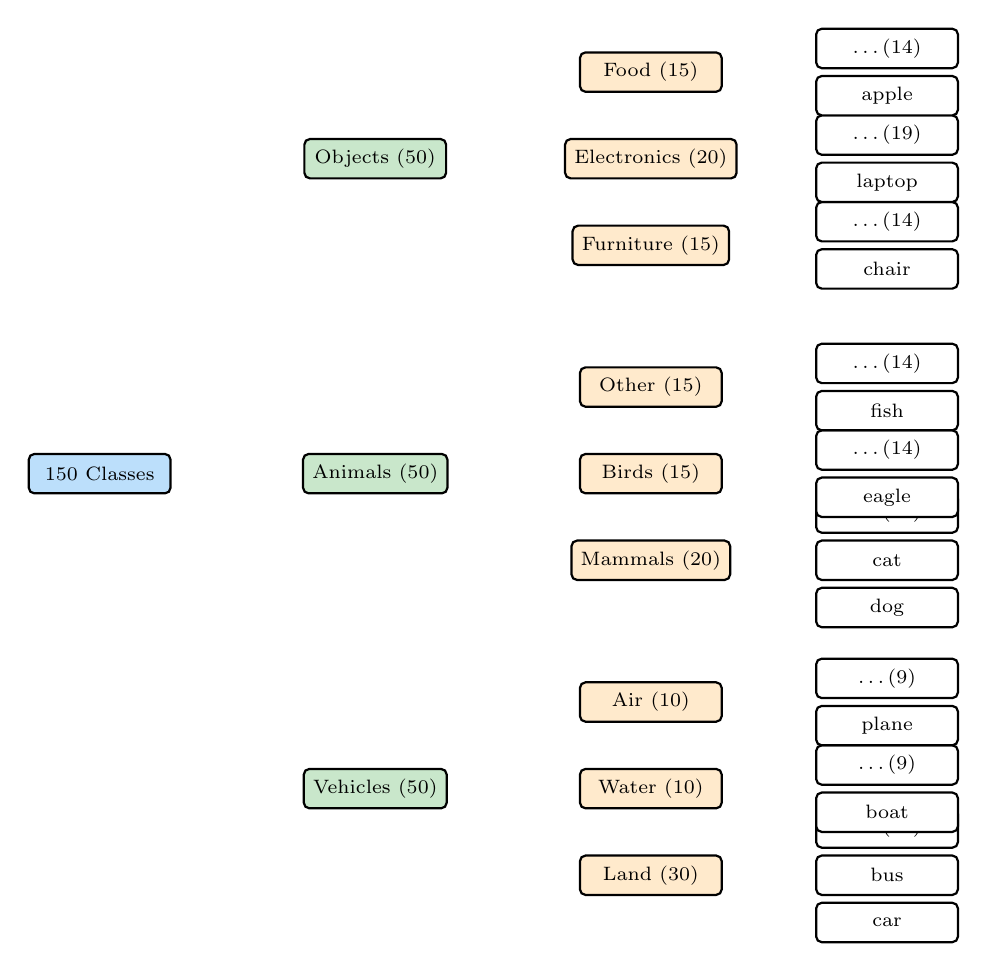
\begin{tikzpicture}[
    grow=right,
    level 1/.style={sibling distance=4.0cm, level distance=3.5cm},
    level 2/.style={sibling distance=1.1cm, level distance=3.5cm},
    level 3/.style={sibling distance=0.6cm, level distance=3.0cm},
    every node/.style={
        rectangle, rounded corners=2pt, draw, thick,
        font=\scriptsize, text centered,
        minimum width=1.8cm, minimum height=0.5cm,
    },
    edge from parent/.style={-Stealth, thick}
]
\node[fill=tikzblue!30] {150 Classes}
    child { node[fill=tikzgreen!30] {Vehicles (50)}
        child { node[fill=tikzorange!20] {Land (30)}
            child { node[fill=white] {car} }
            child { node[fill=white] {bus} }
            child { node[fill=white] {\ldots(28)} }
        }
        child { node[fill=tikzorange!20] {Water (10)}
            child { node[fill=white] {boat} }
            child { node[fill=white] {\ldots(9)} }
        }
        child { node[fill=tikzorange!20] {Air (10)}
            child { node[fill=white] {plane} }
            child { node[fill=white] {\ldots(9)} }
        }
    }
    child { node[fill=tikzgreen!30] {Animals (50)}
        child { node[fill=tikzorange!20] {Mammals (20)}
            child { node[fill=white] {dog} }
            child { node[fill=white] {cat} }
            child { node[fill=white] {\ldots(18)} }
        }
        child { node[fill=tikzorange!20] {Birds (15)}
            child { node[fill=white] {eagle} }
            child { node[fill=white] {\ldots(14)} }
        }
        child { node[fill=tikzorange!20] {Other (15)}
            child { node[fill=white] {fish} }
            child { node[fill=white] {\ldots(14)} }
        }
    }
    child { node[fill=tikzgreen!30] {Objects (50)}
        child { node[fill=tikzorange!20] {Furniture (15)}
            child { node[fill=white] {chair} }
            child { node[fill=white] {\ldots(14)} }
        }
        child { node[fill=tikzorange!20] {Electronics (20)}
            child { node[fill=white] {laptop} }
            child { node[fill=white] {\ldots(19)} }
        }
        child { node[fill=tikzorange!20] {Food (15)}
            child { node[fill=white] {apple} }
            child { node[fill=white] {\ldots(14)} }
        }
    }
;
\end{tikzpicture}
\caption{Example 3-level class hierarchy for 150 leaf classes. Three super-categories
         (\emph{Vehicles}, \emph{Animals}, \emph{Objects}) each contain 5 mid-categories,
         and each mid-category contains 10 leaf classes.}
\label{fig:hierarchy}
\end{figure}

% -------------------------------------------------------
\section{Step 3: Annotation Guidelines}
% -------------------------------------------------------

Use LabelMe or CVAT to produce COCO JSON annotations.
Minimum bounding-box size: 32\,$\times$\,32\,px. Allow at most 5\,px padding per
side. Objects with more than 50\% occlusion should be flagged as \texttt{iscrowd~=~1}.

\begin{lstlisting}[style=bash, caption={Launch LabelMe for annotation}]
labelme --autosave --nodata --output /data/annotations
\end{lstlisting}

% -------------------------------------------------------
\section{Step 4: Converting Annotations to TFRecord}
% -------------------------------------------------------

\begin{lstlisting}[style=bash, caption={Run prepare\_dataset.py with COCO input}]
python src/prepare_dataset.py \
    --input_format coco \
    --annotations  /data/annotations/instances_all.json \
    --images_dir   /data/raw_images \
    --output_dir   /data/tfrecords \
    --splits 0.70 0.15 0.15 \
    --shards 32
\end{lstlisting}

The script performs a stratified train/val/test split, validates minimum per-class
counts, and writes sharded TFRecord files and \texttt{class\_map.json}.

% -------------------------------------------------------
\section{Step 5: Model Architecture Configuration}
% -------------------------------------------------------

\subsection{EfficientDet-Lite Model Comparison}

\begin{table}[ht]
\centering
\caption{EfficientDet-Lite variant comparison. Latency measured on a Pixel~6
         (CPU single-thread). COCO mAP is on the COCO 2017 val set.}
\label{tab:models}
\begin{tabular}{@{}lcccc@{}}
\toprule
\textbf{Model}       & \textbf{Input Size} & \textbf{Params} & \textbf{COCO mAP} & \textbf{CPU Latency} \\
\midrule
EfficientDet-Lite0   & 320\,$\times$\,320  & 3.4\,M  & 26.4\%  & 37\,ms  \\
EfficientDet-Lite1   & 384\,$\times$\,384  & 4.4\,M  & 31.5\%  & 49\,ms  \\
EfficientDet-Lite2   & 512\,$\times$\,512  & 5.3\,M  & 36.0\%  & 69\,ms  \\
EfficientDet-Lite3   & 640\,$\times$\,640  & 7.9\,M  & 39.9\%  & 116\,ms \\
\bottomrule
\end{tabular}
\end{table}

For 150 classes, \textbf{EfficientDet-Lite2} is the recommended baseline.
The 512\,$\times$\,512 input provides better resolution for small objects and
fine-grained classes without being too slow for mobile deployment.

\subsection{Key Configuration Snippet}

\begin{lstlisting}[style=yaml, caption={training\_config.yaml (abridged)}]
model:
  architecture: efficientdet_lite2
  num_classes: 150
  input_image_shape: [512, 512, 3]
  backbone_pretrained: true

training:
  epochs: 100
  batch_size: 16
  learning_rate: 0.08
  lr_warmup_epochs: 5
  mixed_precision: true
  early_stopping:
    enabled: true
    patience: 15

export:
  tflite_filename: best_model.tflite
  quantisation: dynamic_range
\end{lstlisting}

% -------------------------------------------------------
\section{Step 6: Launching Training}
% -------------------------------------------------------

\begin{lstlisting}[style=bash, caption={Start training}]
python src/train_model.py \
    --config     configs/training_config.yaml \
    --output_dir /models/efficientdet_lite2_150cls
\end{lstlisting}

The script will:
\begin{enumerate}[nosep]
    \item Enable mixed-precision training.
    \item Load train/val TFRecord datasets.
    \item Initialise EfficientDet-Lite2 with ImageNet pre-trained weights.
    \item Train with cosine LR decay and early stopping.
    \item Export the best checkpoint to TFLite.
\end{enumerate}

% -------------------------------------------------------
\section{Step 7: Monitoring with TensorBoard}
% -------------------------------------------------------

\begin{lstlisting}[style=bash, caption={Launch TensorBoard}]
tensorboard --logdir /models/efficientdet_lite2_150cls/logs --port 6006
\end{lstlisting}

Key metrics: \texttt{val\_AP} (primary), \texttt{val\_loss}, \texttt{box\_loss},
\texttt{cls\_loss}. A healthy training run shows \texttt{val\_AP} increasing
steadily for the first 40--60 epochs before plateauing.

% -------------------------------------------------------
\section{Step 8: Evaluating the Model}
% -------------------------------------------------------

\begin{lstlisting}[style=bash, caption={Run evaluation on the test split}]
python src/evaluate_model.py \
    --model     /models/efficientdet_lite2_150cls/best_model.tflite \
    --dataset   /data/tfrecords/test \
    --class_map /data/tfrecords/class_map.json \
    --output_dir /reports
\end{lstlisting}

The script computes:
\begin{itemize}[nosep]
    \item mAP@0.5 and mAP@0.5:0.95 (COCO-style)
    \item Per-class precision, recall, and F1 (top-20 and bottom-20 by F1)
    \item Confusion matrix saved as \texttt{confusion\_matrix.png}
\end{itemize}

% -------------------------------------------------------
\section{Step 9: Exporting to TFLite}
% -------------------------------------------------------

\begin{lstlisting}[style=python, caption={Dynamic-range quantisation export}]
import tensorflow as tf

converter = tf.lite.TFLiteConverter.from_saved_model(
    "/models/efficientdet_lite2_150cls/saved_model"
)
converter.optimizations = [tf.lite.Optimize.DEFAULT]
tflite_model = converter.convert()

with open("best_model.tflite", "wb") as f:
    f.write(tflite_model)
print(f"Model size: {len(tflite_model) / 1024**2:.1f} MB")
\end{lstlisting}

Dynamic-range quantisation reduces model size by approximately 3--4$\times$ with
less than 1\% mAP drop on most datasets.

% -------------------------------------------------------
\section{Step 10: Integrating with MediaPipe}
% -------------------------------------------------------

\begin{lstlisting}[style=python, caption={Run inference with MediaPipe Tasks API}]
import mediapipe as mp
from mediapipe.tasks import python as mp_python
from mediapipe.tasks.python import vision

options = vision.ObjectDetectorOptions(
    base_options=mp_python.BaseOptions(
        model_asset_path="best_model_with_metadata.tflite"
    ),
    running_mode=vision.RunningMode.IMAGE,
    max_results=50,
    score_threshold=0.3,
)

with vision.ObjectDetector.create_from_options(options) as detector:
    image = mp.Image.create_from_file("test_image.jpg")
    result = detector.detect(image)
    for det in result.detections:
        cat = det.categories[0]
        print(f"{cat.category_name}: {cat.score:.2f}")
\end{lstlisting}

% -------------------------------------------------------
\section{Troubleshooting}
% -------------------------------------------------------

\begin{description}
    \item[OOM on GPU] Reduce \texttt{batch\_size} to 8 in the config.
    \item[NaN loss] Reduce learning rate to 0.04 and increase warmup to 10 epochs.
    \item[mAP stuck below 0.10] Verify TFRecord annotations with
        \texttt{visualise\_dataset.py}; check class\_map.json index continuity.
    \item[Zero AP for some classes] Verify those classes have $\ge$50 validation
        images and that their COCO category ID is not~0.
    \item[Fine-grained classes have low AP] Increase data to 700--1\,000 images/class,
        use EfficientDet-Lite3 (640$\times$640), or apply copy-paste augmentation.
\end{description}

% -------------------------------------------------------
\end{document}
